\documentclass{article}

\usepackage[utf8]{inputenc}
\usepackage[brazil]{babel}

\title{Avaliação de Reconhecimento de Padrões}
\author{Rúbia Reis Guerra \\ 2013031143}

\usepackage{Sweave}
\begin{document}
\Sconcordance{concordance:prova.tex:prova.Rnw:%
1 8 1 1 0 4 1 1 2 1 0 6 1 1 11 13 0 1 2 1 1 1 2 1 0 6 1 1 3 5 0 1 2 1 1 %
1 2 1 0 5 1 9 0 1 1 4 0 1 2 1 1 1 6 5 0 1 1 1 5 8 0 1 2 1 1 1 6 5 0 1 1 %
1 5 8 0 1 2 3 1 1 4 3 0 4 1 7 0 2 2 7 0 1 2 1 4 3 0 1 5 4 0 1 1 24 0 1 %
2 8 1 1 4 3 0 1 1 4 0 1 2 3 1 1 2 1 0 6 1 1 2 1 4 3 0 1 9 6 0 1 1 30 0 %
1 2 2 1 1 2 1 0 6 1 1 2 1 4 3 0 1 9 6 0 1 1 30 0 1 2 2 1}

\maketitle

\section{Pacotes utilizados}
\begin{Schunk}
\begin{Sinput}
> rm(list=ls())
> library('mclust')
> ###########################
> # Auxiliares #
> tp <- c()
> fp <- c()
> fn <- c()
> prec <- c()
> rec <- c()
> f1 <- c()
> error <- c()
> mse <- c()
> sde <- c()
\end{Sinput}
\end{Schunk}

\section{Análise dos dados}
\begin{Schunk}
\begin{Sinput}
> bupa <- as.matrix(read.csv("bupa.data", header=FALSE))
> X <- bupa[,(1:6)] # dados de entrada
> Y <- as.matrix(2*(bupa[,7]-1.5)) # rotulos das classes como [-1,+1]
> i_cm1 <- which(Y == -1) # amostras da classe -1
> i_c1 <- which(Y == 1) # amostras da classe +1
> Nm1 <- length(i_cm1) # tamanho da classe -1
> N1 <- length(i_c1) # tamanho da classe +1
> ## Analise dos dados
> clPairs(bupa, Y) ## Analise 
> cor(bupa) ## Calculo da correlacao
\end{Sinput}
\begin{Soutput}
            V1          V2          V3        V4        V5          V6
V1  1.00000000  0.04410300  0.14769505 0.1877652 0.2223145  0.31267960
V2  0.04410300  1.00000000  0.07620761 0.1460565 0.1331404  0.10079606
V3  0.14769505  0.07620761  1.00000000 0.7396749 0.5034353  0.20684793
V4  0.18776515  0.14605655  0.73967487 1.0000000 0.5276259  0.27958777
V5  0.22231449  0.13314040  0.50343525 0.5276259 1.0000000  0.34122396
V6  0.31267960  0.10079606  0.20684793 0.2795878 0.3412240  1.00000000
V7 -0.09107012 -0.09805018 -0.03500879 0.1573558 0.1463925 -0.02204853
            V7
V1 -0.09107012
V2 -0.09805018
V3 -0.03500879
V4  0.15735580
V5  0.14639252
V6 -0.02204853
V7  1.00000000
\end{Soutput}
\begin{Sinput}
> 
\end{Sinput}
\end{Schunk}
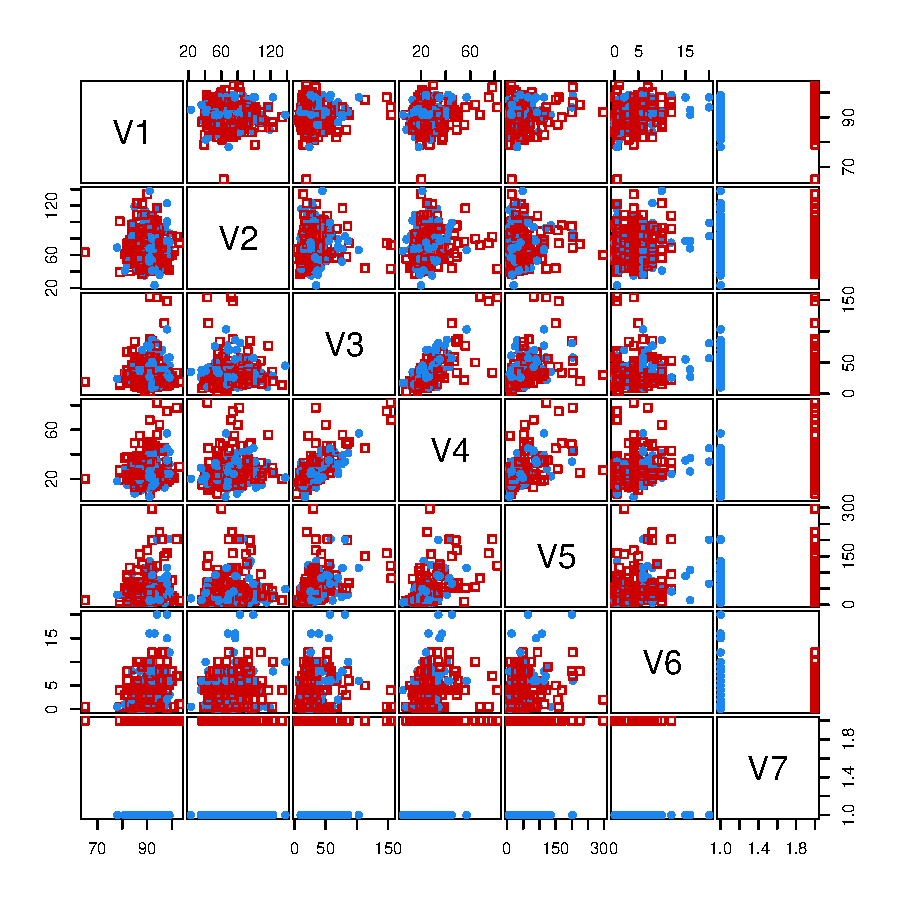
\includegraphics{prova-002}

Como pode ser observado no plot gerado, existe um alto grau de correlação entre as variáveis de entrada e, como consequência, ocorre a sobreposição das classes. Podemos assumir que se trata de um problema multi-modal com características de separacão não-lineares e tentar resolvê-lo por um modelo de misturas normais.

\section{Coerência da rotulação}
Para analisar a coerência entre os agrupamentos gerados pelo método de clustering e os rótulos de cada classe, utilizou-se o pacote \textit{mclust} e, em sequência, foi obtida a distribuição dos padrões da classes dentro dos agrupamentos.
\begin{Schunk}
\begin{Sinput}
> mod = Mclust(X) # Clustering
> table(mod$classification, Y) # Clusters x Classes
\end{Sinput}
\begin{Soutput}
   Y
    -1  1
  1 53 82
  2 72 80
  3 18 35
  4  2  3
\end{Soutput}
\begin{Sinput}
> plot(mod, what = "classification") # Visualização dos agrupamentos
\end{Sinput}
\end{Schunk}
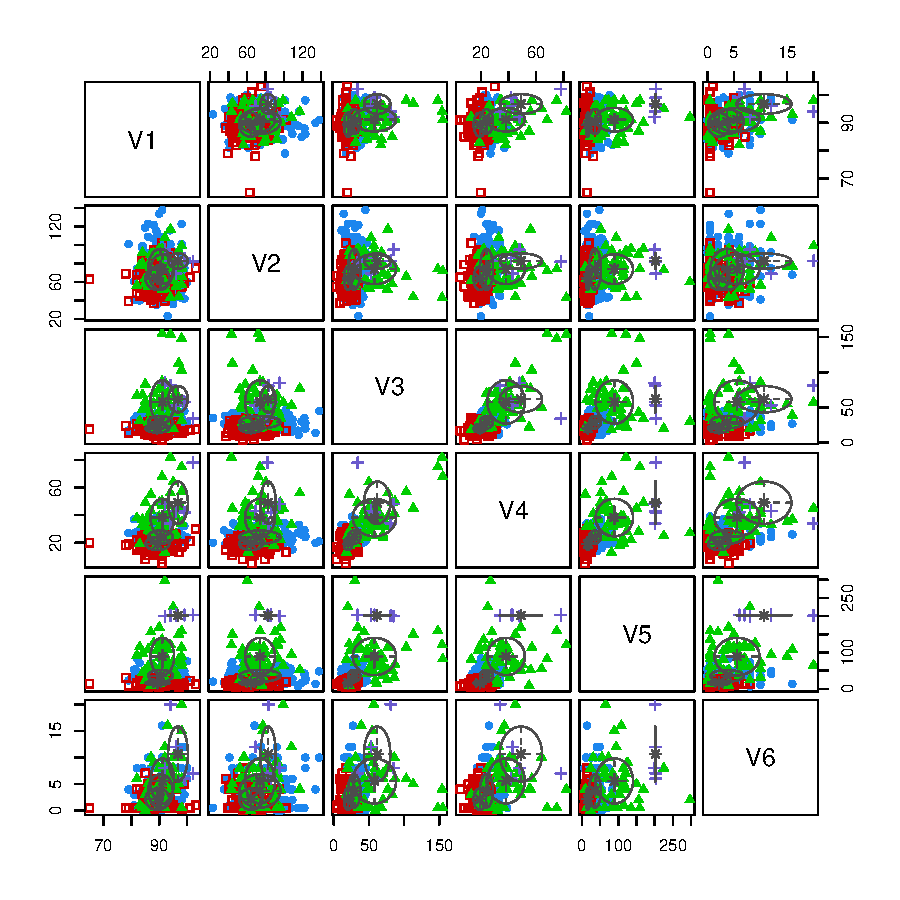
\includegraphics{prova-003}

Observamos que não há relação direta entre os rótulos das classes e os agrupamentos obtidos pelo algoritmo Kmédias. Os padrões foram distribuídos entre os 4 agrupamentos de forma que não necessariamente exemplos de uma mesma classe pertencem ao mesmo cluster. Esta observação é coerente, pois como analisado no item anterior, a correlação entre os atributos de entrada é significativa e as classes se sobrepõem espacialmente.

\section{Classificação}
O problema de classificação foi tratado utilizando-se um classificador Bayesiano. As probabilidades a priori foram calculadas a partir da quantidade de amostras de cada classe e as densidades de probabilidade foram encontradas utilizando-se um modelo de mistura de gaussianas, obtido pelo algoritmo K-médias.
\begin{Schunk}
\begin{Sinput}
> for(j in 1:10){
+   ###########################
+   # Partição entre treino e teste #
+   index <- sample(2, nrow(bupa), replace=TRUE, prob=c(0.70,0.30))
+   
+   ###########################
+   # Conjunto de treinamento #
+   training <- X[which(index==1),]
+   trainingLabels <- as.matrix(Y[which(index==1)])
+   
+   ###########################
+   # Conjunto de teste #
+   test <- X[which(index==2),]
+   testLabels <- as.matrix(Y[which(index==2)])
+   
+   ###########################
+   # Probabilidades a priori #
+   pc1 <- Nm1/(Nm1+N1)
+   pc2 <- N1/(Nm1+N1)
+   
+   ###########################
+   # Treinamento #
+   mod1 = densityMclust(training[which(trainingLabels==(-1)),])
+   mod2 = densityMclust(training[which(trainingLabels==1),])
+   
+   ###########################
+   # Teste #
+   pxc1 <- dens(modelName=mod1$modelName, data = test, parameters = mod1$parameters)
+   pxc2 <- dens(modelName=mod2$modelName, data = test, parameters = mod2$parameters)
+   
+   ###########################
+   # Classificação #
+   Ntest <- dim(test)[1]
+   testY <- c()
+   for(i in 1:Ntest)
+   {
+     testY[i] <- ifelse(pxc1[i]/pxc2[i] >= pc2/pc1, -1, 1)
+     error[i] <- (testY[i]-testLabels[i])^2
+   }
+   
+   # MSE e SD #
+   mse[j] <- mean(error)
+   sde[j] <- sd(error)
+   
+   # Matriz de confusão #
+   testCM <- table(testY,testLabels)
+   
+   # Precision, recall, F1 #
+   tp[j] <- sum((testY==(-1)) & (testLabels==(-1))) # True positives
+   fp[j] <- sum((testY==(-1)) & (testLabels==1)) # False positives
+   fn[j] <- sum((testY==1) & (testLabels==(-1))) # False negatives
+   prec[j] <- tp[j]/(tp[j] + fp[j]) # Precision
+   rec[j] <- tp[j]/(tp[j] + fn[j]) # Recall
+   f1[j] <- 2*prec[j]*rec[j]/(prec[j]+rec[j]) # F1 Score
+ }
> mean(mse) # MSE
\end{Sinput}
\begin{Soutput}
[1] 1.36
\end{Soutput}
\begin{Sinput}
> mean(sde) # SD
\end{Sinput}
\begin{Soutput}
[1] 1.887346
\end{Soutput}
\end{Schunk}
Analisando o desempenho do classificador após 10 iterações, conclui-se que a Regra de Bayes separa as duas classes de forma coerente.

\end{document}
